% Finding the Leak -- DPL 2026, Question 1. CVPR author-kit format.
% Every number is a macro from numbers.tex and every table body from tables.tex
% (both written by scripts/make_numbers.R); figures come from ../outputs/figures.
\documentclass[10pt,twocolumn,letterpaper]{article}
\usepackage[pagenumbers]{cvpr}
\usepackage{graphicx,booktabs,amsmath,amssymb,xcolor}
\usepackage{cuted}
\usepackage{caption}
\definecolor{cvprblue}{rgb}{0.21,0.49,0.74}
\usepackage[breaklinks,colorlinks,allcolors=cvprblue]{hyperref}
\graphicspath{{../outputs/figures/}}
% generated by scripts/make_numbers.R - do not edit
\makeatletter
\@namedef{kv@team}{Royal Challengers Bengaluru}
\@namedef{kv@teamabbr}{RCB}
\@namedef{kv@home}{Chinnaswamy}
\@namedef{kv@rows}{34,967}
\@namedef{kv@cols}{61}
\@namedef{kv@matches}{145}
\@namedef{kv@venues}{14}
\@namedef{kv@legalballs}{33,612}
\@namedef{kv@truewickets}{1,797}
\@namedef{kv@batoutpct}{99.9}
\@namedef{kv@wagonagree}{99.2}
\@namedef{kv@pricedplayerseasons}{399}
\@namedef{kv@rr2023}{8.94}
\@namedef{kv@rr2024}{9.52}
\@namedef{kv@ppd}{0.75}
\@namedef{kv@midd}{0.41}
\@namedef{kv@dthd}{0.74}
\@namedef{kv@venuegap}{1.8}
\@namedef{kv@wincormetric}{Bowling wickets per over (MID)}
\@namedef{kv@wincorr}{0.69}
\@namedef{kv@spinmidshare23}{62}
\@namedef{kv@spinmidshare24}{54}
\@namedef{kv@spinmidecon24}{8.22}
\@namedef{kv@pacemidecon24}{9.29}
\@namedef{kv@teambought23}{7}
\@namedef{kv@teambought24}{39.7}
\@namedef{kv@kpyth}{7.92}
\@namedef{kv@pythr2}{0.54}
\@namedef{kv@ng1}{2}
\@namedef{kv@g1teamsa}{RCB}
\@namedef{kv@g1teamsb}{PBKS}
\@namedef{kv@g1teamslist}{RCB and PBKS}
\@namedef{kv@gap2023}{\ensuremath{-}5.4}
\@namedef{kv@gap2024}{\ensuremath{-}10.9}
\@namedef{kv@winsshort}{\ensuremath{-}2.4}
\@namedef{kv@pbothbelow}{58}
\@namedef{kv@celllabel}{Bowling: middle overs spin}
\@namedef{kv@cellper100}{\ensuremath{-}27.9}
\@namedef{kv@celllo}{\ensuremath{-}48.5}
\@namedef{kv@cellhi}{\ensuremath{-}5.7}
\@namedef{kv@cellq}{0.061}
\@namedef{kv@cellground}{\ensuremath{-}23}
\@namedef{kv@cellgroundp}{0.0014}
\@namedef{kv@cell2023}{\ensuremath{-}26.8}
\@namedef{kv@cell2024}{\ensuremath{-}29}
\@namedef{kv@ncells}{83}
\@namedef{kv@nthree}{1}
\@namedef{kv@nprobable}{4}
\@namedef{kv@ng3}{5}
\@namedef{kv@surplus}{\ensuremath{-}11.7}
\@namedef{kv@crperwarteam23}{8.81}
\@namedef{kv@leaguecpwa}{6.15}
\@namedef{kv@leaguecpwb}{5.93}
\@namedef{kv@spendr}{0.36}
\@namedef{kv@spendp}{0.12}
\@namedef{kv@warwinr}{0.7}
\@namedef{kv@npassall}{1}
\@namedef{kv@rankbowlpp}{1}
\@namedef{kv@rankbowldth}{1}
\@namedef{kv@rankbowlmid}{10}
\@namedef{kv@rankbowlspin}{10}
\@namedef{kv@rankbatpp}{2}
\@namedef{kv@warwinsr}{0.75}
\@namedef{kv@m2gain}{2.08}
\@namedef{kv@m2calib}{1.004}
\@namedef{kv@m4gain}{2.73}
\@namedef{kv@w1logloss}{0.508}
\@namedef{kv@w3logloss}{0.526}
\@namedef{kv@w4logloss}{0.554}
\@namedef{kv@rpw}{90.3}
\@namedef{kv@kbowl}{585}
\@namedef{kv@kbat}{456}
\@namedef{kv@overseaspremium}{170}
\@namedef{kv@venuecoefraw}{5.3}
\@namedef{kv@venuecoeffe}{\ensuremath{-}0.6}
\@namedef{kv@midspin}{\ensuremath{-}24.1}
\@namedef{kv@leaguespin}{3.8}
\@namedef{kv@nextworst}{\ensuremath{-}8.2}
\@namedef{kv@goodplayersa}{Cameron Green}
\@namedef{kv@goodplayersb}{Mohammed Siraj}
\@namedef{kv@goodplayersc}{Glenn Maxwell}
\@namedef{kv@goodplayerslist}{Cameron Green, Mohammed Siraj and Glenn Maxwell}
\@namedef{kv@goodshare}{23}
\@namedef{kv@medreg}{2.3}
\@namedef{kv@ownspina}{Karn Sharma}
\@namedef{kv@ownspinb}{Wanindu Hasaranga}
\@namedef{kv@ownspinc}{Mayank Dagar}
\@namedef{kv@ownspinlist}{Karn Sharma, Wanindu Hasaranga and Mayank Dagar}
\@namedef{kv@closeW}{0}
\@namedef{kv@closeM}{3}
\@namedef{kv@otherW}{14}
\@namedef{kv@otherM}{26}
\@namedef{kv@clutchrbat}{\ensuremath{-}0.28}
\@namedef{kv@clutchrbowl}{\ensuremath{-}0.24}
\@namedef{kv@cvflagged}{11}
\@namedef{kv@cvsurvive}{2}
\@namedef{kv@surplus23}{\ensuremath{-}19.7}
\@namedef{kv@surplus24}{8.1}
\@namedef{kv@stakerunsa}{105}
\@namedef{kv@stakerunsb}{103}
\@namedef{kv@stakewinsa}{1.2}
\@namedef{kv@stakewinsb}{1.1}
\@namedef{kv@stakecra}{7.2}
\@namedef{kv@stakecrb}{6.7}
\@namedef{kv@pacenew}{36.2}
\@namedef{kv@spinnew}{2}
\@namedef{kv@pacenewnames}{Alzarri Joseph, Cameron Green, Lockie Ferguson, Vijaykumar Vyshak, Yash Dayal}
\@namedef{kv@spinnewnames}{Mayank Dagar, Swapnil Singh}
\@namedef{kv@releasedspina}{Shahbaz Ahmed}
\@namedef{kv@releasedspinb}{Wanindu Hasaranga}
\@namedef{kv@releasedspinlist}{Shahbaz Ahmed and Wanindu Hasaranga}
\@namedef{kv@releasedspincr}{13.15}
\@namedef{kv@toptrade}{Cameron Green}
\@namedef{kv@toptradecr}{17.5}
\@namedef{kv@topbuy}{Alzarri Joseph}
\@namedef{kv@topbuycr}{11.5}
\@namedef{kv@topbuywar}{0}
\@namedef{kv@wararrived24}{4.6}
\@namedef{kv@warreleased24}{2}
\@namedef{kv@cpwarrived24}{8.72}
\@namedef{kv@spin24top}{Karn Sharma}
\@namedef{kv@spin24topshare}{39}
\@namedef{kv@spin24topecon}{10}
\@namedef{kv@marketpooln}{6}
\@namedef{kv@besthindplayer}{Axar Patel}
\@namedef{kv@besthindruns}{138}
\@namedef{kv@besthindwins}{1.5}
\@namedef{kv@besthindcr}{9}
\@namedef{kv@foremaxwins}{0.23}
\@namedef{kv@elWa}{1}
\@namedef{kv@elWb}{6}
\@namedef{kv@elMa}{7}
\@namedef{kv@elMb}{7}
\@namedef{kv@elrrfora}{9.55}
\@namedef{kv@elrrforb}{11.01}
\@namedef{kv@elrragainsta}{10.7}
\@namedef{kv@elrragainstb}{9.16}
\@namedef{kv@elppwktsa}{4}
\@namedef{kv@elppwktsb}{18}
\@namedef{kv@elmidspinecona}{10.12}
\@namedef{kv@elmidspineconb}{9.06}
\@namedef{kv@optA}{0.07}
\@namedef{kv@optB}{0.14}
\@namedef{kv@optC}{0.24}
\@namedef{kv@optCp}{85}
\@namedef{kv@optD}{0.44}
\@namedef{kv@histupper}{0.8}
\@namedef{kv@q75reg}{5.7}
\@namedef{kv@rnow}{\ensuremath{-}2.6}
\@namedef{kv@shortlista}{Varun Chakravarthy}
\@namedef{kv@shortlistb}{Axar Patel}
\@namedef{kv@shortlistc}{Krunal Pandya}
\@namedef{kv@shortlistd}{Harpreet Brar}
\@namedef{kv@shortliste}{Ravichandran Ashwin}
\@namedef{kv@shortlistf}{Kuldeep Yadav}
\@namedef{kv@shortlistlist}{Varun Chakravarthy, Axar Patel, Krunal Pandya, Harpreet Brar, Ravichandran Ashwin and Kuldeep Yadav}
\@namedef{kv@corea}{Yash Dayal}
\@namedef{kv@coreb}{Mohammed Siraj}
\@namedef{kv@corec}{Dinesh Karthik}
\@namedef{kv@cored}{Rajat Patidar}
\@namedef{kv@coree}{Faf du Plessis}
\@namedef{kv@corelist}{Yash Dayal, Mohammed Siraj, Dinesh Karthik, Rajat Patidar and Faf du Plessis}
\@namedef{kv@reviewa}{Glenn Maxwell}
\@namedef{kv@reviewb}{Alzarri Joseph}
\@namedef{kv@reviewlist}{Glenn Maxwell and Alzarri Joseph}
\newcommand{\kv}[1]{\@nameuse{kv@#1}}
\makeatother

% generated by scripts/make_numbers.R - do not edit
\newcommand{\gatesrows}{
RCB & \ensuremath{-}5.4 & \ensuremath{-}10.9 & Bowling middle overs spin & \ensuremath{-}27.9 & 3 & \ensuremath{-}11.7 & 3 \\
PBKS & \ensuremath{-}6.5 & \ensuremath{-}4.7 & Batting middle overs spin & \ensuremath{-}9.4 & 1 & \ensuremath{-}9.2 & 2 \\
LSG & 10.8 & 3.0 & Batting powerplay pace & \ensuremath{-}9.2 & 2 & \ensuremath{-}9.3 & 1 \\
DC & 5.4 & 13.7 & Batting death overs pace & \ensuremath{-}17.3 & 2 & \ensuremath{-}8.2 & 1 \\
SRH & \ensuremath{-}12.6 & 3.9 & Batting middle overs pace & \ensuremath{-}11.4 & 1 & \ensuremath{-}8.4 & 1 \\
MI & 6.9 & \ensuremath{-}14.5 & Bowling middle overs spin & \ensuremath{-}10.5 & 2 & 3.7 & 0 \\
GT & 0.7 & \ensuremath{-}2.5 & Batting middle overs pace & \ensuremath{-}14.7 & 2 & 11.1 & 0 \\
CSK & 8.6 & \ensuremath{-}8.7 & Bowling powerplay pace & \ensuremath{-}8.2 & 1 & 4.6 & 0 \\
RR & \ensuremath{-}2.5 & 10.7 & Batting middle overs pace & \ensuremath{-}12.2 & 1 & 0.8 & 0 \\
KKR & \ensuremath{-}6.6 & 9.3 & Bowling powerplay pace & \ensuremath{-}10.3 & 0 & 26.5 & 0 \\
}
\newcommand{\elrows}{
M0 global mean & 0.00 & -- \\
M1 cell means (over x wickets) & 1.20 & 0.824 \\
M2 log-linear + EB shrinkage & 2.08 & 1.004 \\
M3 hierarchical GLMM & 1.29 & 0.763 \\
M4 gradient boosting & 2.73 & 0.823 \\
}
\newcommand{\wprows}{
W0 Null (base rate) & 0.500 & 0.250 & 0.693 \\
W1 Resource curve + Pythagorean (n = 6) & 0.829 & 0.170 & 0.508 \\
W2 Resource curve + fitted exponent & 0.829 & 0.175 & 0.521 \\
W3 Logistic, splines & 0.811 & 0.179 & 0.526 \\
W4 GAM, tensor surface & 0.794 & 0.184 & 0.554 \\
}
\newcommand{\oprows}{
A. Redeploy only (free) & 0.07 & \ensuremath{-}0.09 & 0.22 & 76 \\
B. Median regular spinner & 0.14 & \ensuremath{-}0.23 & 0.52 & 73 \\
C. Top-quartile Indian spinner & 0.24 & \ensuremath{-}0.14 & 0.61 & 85 \\
D. Elite spinner (best in league) & 0.44 & 0.05 & 0.82 & 97 \\
}
\newcommand{\hyrows}{
H1 & Shortfall sits in one cell & Supported \\
H2 & Deployment problem & Partly supported \\
H3 & Squad-building problem & Supported \\
H4 & Venue artefact & Supported (bowling overall) \\
H5 & Money in the wrong roles & Supported (2023) \\
H6 & Pressure, not level & Rejected \\
H7 & Auction did not address 2023 & Supported \\
H8 & 2024 turn came elsewhere & Supported \\
}

\def\paperID{DPL-Q1}
\def\confName{DPL}
\def\confYear{2026}

\title{Finding the Leak: Choosing a Franchise Fairly and Auditing Its Decisions\\with Ball-by-Ball IPL Data}
\author{Faizan Khan\\
Data Premier League 2026 -- Preliminary Round, Question 1\\
{\tt\small github.com/sportsanalystf/data-premier-league-26}}

\begin{document}
\twocolumn[{%
\renewcommand\twocolumn[1][]{#1}%
\maketitle
\begin{center}
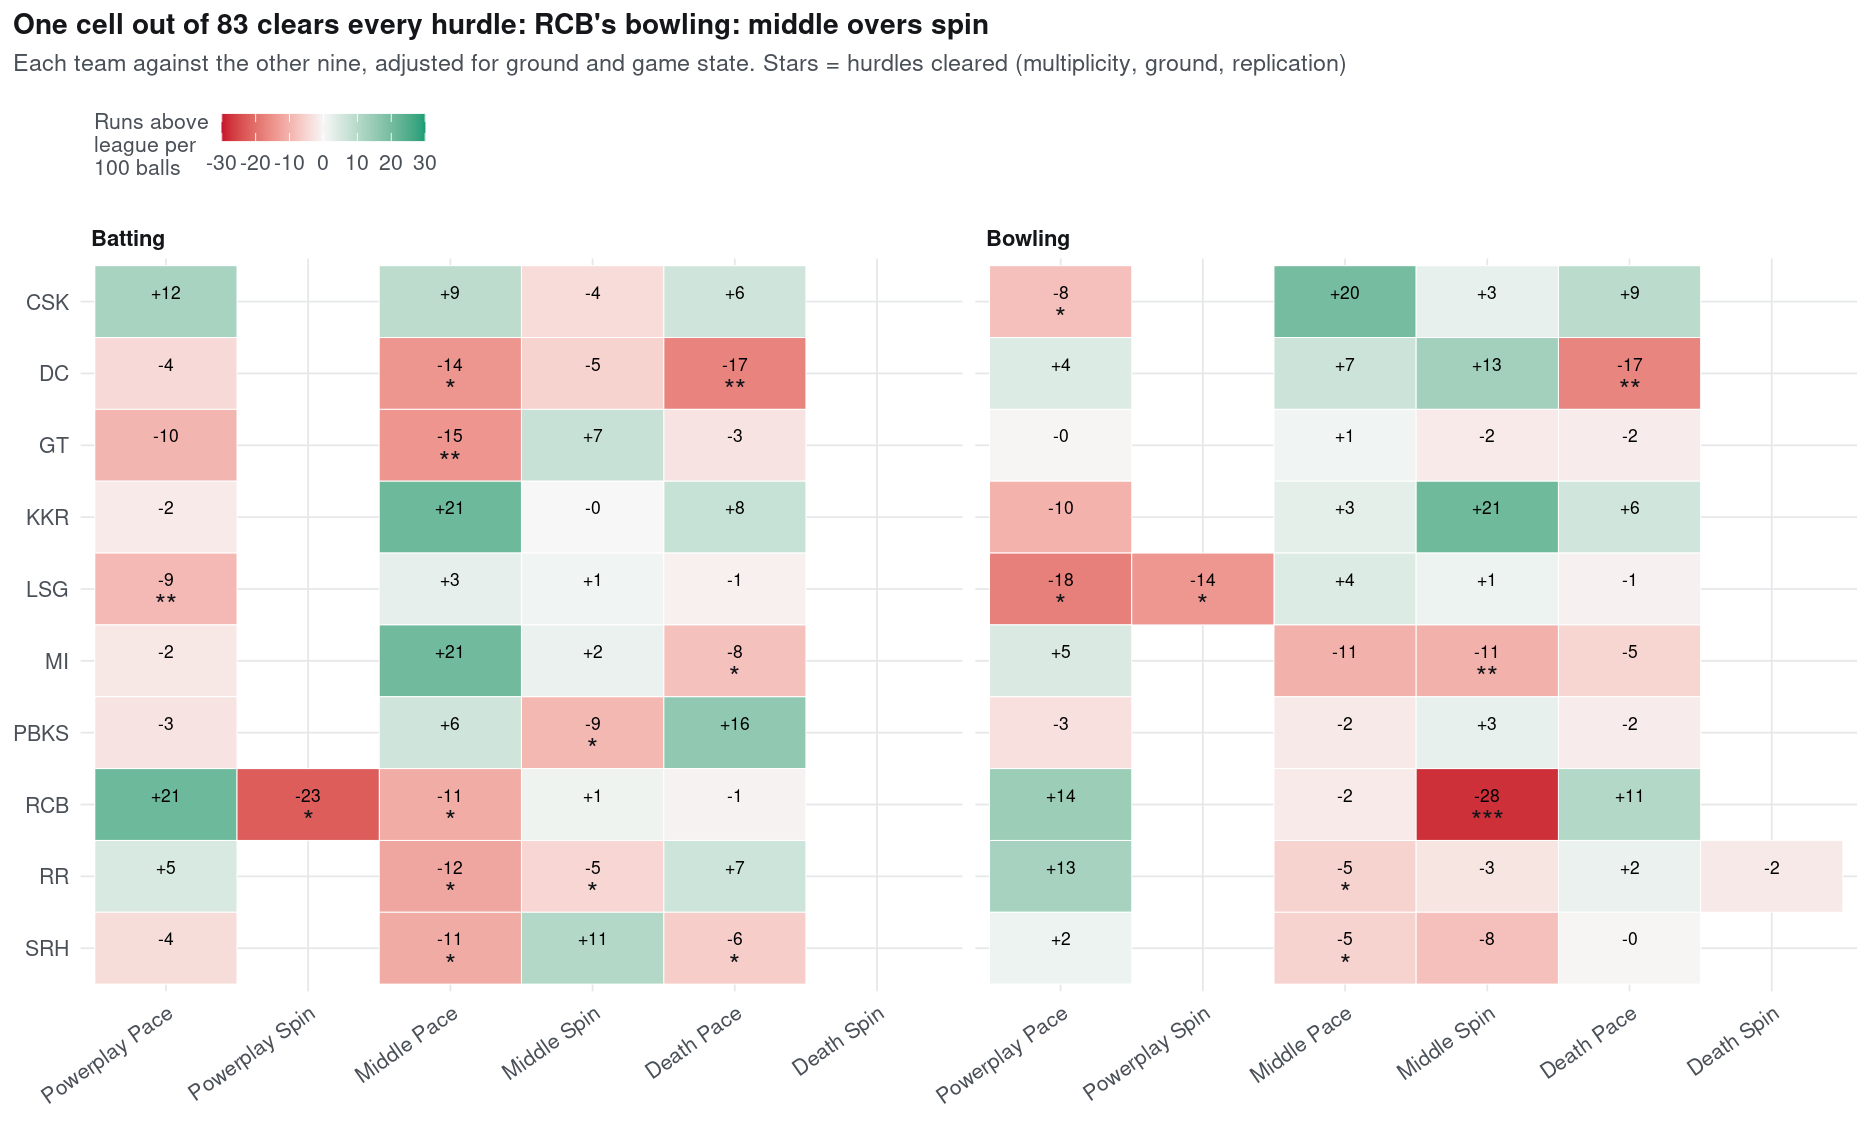
\includegraphics[width=0.94\textwidth]{a05_cell_scan.png}
\captionof{figure}{Every team, every cell: runs above the rest of the league per 100 balls for batting and bowling by phase and bowler type, IPL 2023--24, with ground and game state held fixed. Stars count hurdles cleared (multiplicity, ground fixed effects, replication). One of \kv{ncells} team-cells clears all three: \kv{teamabbr}'s middle-overs spin bowling.}
\label{fig:teaser}
\end{center}
\vspace{1em}
}]

\begin{abstract}
A franchise report has two problems inside it: which team to study, and what that team should do. We answer the first with a screen every team goes through, using three gates fixed in advance: winning fewer games than the runs deserved in both seasons (Pythagorean expectation, $k=\kv{kpyth}$), a weakness on the field that survives a Benjamini--Hochberg correction, ground fixed effects and replication across seasons, and a negative money surplus. Only \kv{team} passes all three. For that team we test eight written hypotheses and audit its decisions season by season. Most of its reputation for poor bowling is its home ground; what remains, and repeats, is middle-overs spin (\kv{cellper100} runs per 100 balls against the rest of the league; \kv{cell2023} in 2023 and \kv{cell2024} in 2024), costing about \kv{stakewinsa} wins a season. After 2023 the franchise released both main spinners and spent INR~\kv{pacenew} crore of new money on pace against INR~\kv{spinnew} crore on spin; its 2024 recovery (\kv{elWa} win in seven, then \kv{elWb}) came from the powerplay, not the weak cell. Four model ladders validated on a later season supply the measurements; in two of them the simplest well-calibrated model wins.
\end{abstract}

\section{Introduction}
A franchise can change three things: who bowls and bats when, who is in the squad, and what it pays. The evidence usually brought to those decisions, economy and strike rates, mixes skill with the home ground, the match situations a team creates and the noise of small samples. Following the mentor guidance for this competition we start from the decision~\cite{desai2026} and work through six steps: situation, search, obvious gap, representation (a problem map from purse to squad to phases to runs to wins and back to the next auction), hypotheses, key question.

Our contributions: (i) a \emph{fair choice of subject}, by gates rather than a composite score; (ii) \emph{model ladders} scored on a later season; (iii) a \emph{decision audit} that separates what the franchise could have known at the time (foresight) from what we know now (hindsight), and prices each step in runs, wins and crore.

\section{Related work}
Run value conditioned on game state underlies cricWAR~\cite{rafique2022}, which chains run value and replacement level into wins above replacement. Ganjoo~\cite{ganjoo2026} treats balls and wickets as resources, links score ratios to win probability with a Pythagorean form and defines leverage as the swing between a six and a wicket. Bandyopadhyay~\cite{bandyopadhyay} fits a multiplicative expectation with empirical-Bayes shrinkage; Date~\cite{date} argues for the batter's balls faced in the expectation; Nielsen~\cite{nielsen} quantifies how slowly T20 rates stabilise. Malhotra~\cite{malhotra2022} fits hedonic auction prices. For multiple comparisons we use Benjamini--Hochberg~\cite{bh1995}; for pressure, the PACE framework~\cite{gupta2026}.

\section{Data}
Ball-by-ball records for IPL 2023 and 2024 (\kv{rows} deliveries, \kv{matches} matches, \kv{venues} venues) with tracking fields, plus both auction sheets (retained, sold, traded, unsold). A \texttt{bat\_out} flag is true on \kv{batoutpct}\% of rows, retirements conflate two outcomes, and wagon zones are undocumented (decoded with \kv{wagonagree}\% agreement). All game state is rebuilt as it stood before each ball and a guard blocks post-delivery features. League scoring rose from \kv{rr2023} to \kv{rr2024} runs an over, mostly in the powerplay (+\kv{ppd}) and death (+\kv{dthd}) rather than the middle overs (+\kv{midd}), so every comparison is made within season. Across the 20 team-seasons the rate most correlated with win percentage is middle-overs bowling wickets per over ($r=\kv{wincorr}$).

\section{Method}
\subsection{Problem A: three gates}
\textbf{G1 Results.} Expected win share is $R^k/(R^k+A^k)$ with $k$ fitted on all team-seasons ($R^2=\kv{pythr2}$). A team passes if it is below expectation in both seasons. \textbf{G2 Cause.} Each team's game is split into 12 cells (discipline $\times$ phase $\times$ pace/spin). The cell value is runs above average per 100 balls (\cref{sec:tools}) for the team minus the other nine; intervals come from a match-cluster bootstrap. A cell must be worse than the league and clear three hurdles: BH $q<0.10$ within the team's grid; a negative team coefficient in a regression of raw runs per ball on season and ground fixed effects with match-clustered errors ($p<0.05$); and a negative value in each season separately. \textbf{G3 Money.} Surplus is squad WAR valued at the league's crore-per-WAR rate minus spend, summed over two seasons.

\subsection{Measuring tools}\label{sec:tools}
Expected runs per ball come from a ladder M0--M4; M2 is $\mu_i=\mu_0\prod_f\hat\gamma_{f,c_f(i)}$ over over, innings, wickets, bowler type, set-ness, venue and handedness, each multiplier shrunk towards one. Win probability uses a resource curve $R(b,w)=R_0(1-e^{-b/\beta})F(w)$ and $P=r^n/(1+r^n)$ with $n=6$ (W1), against fitted, spline-logistic and GAM alternatives. Runs above average add a wicket term $(d_i-\hat p_i)c_i$ priced from the resource curve, and roll up to WAR via a replacement level and runs per win $=4\bar R/k=\kv{rpw}$. Talent rates are shrunk with $\kappa=\kv{kbowl}$ balls (bowling); WAR is not.

\subsection{Problem B: hypotheses and the decision audit}
Eight hypotheses were written with falsifiers before testing (\cref{tab:hyp}). The audit follows the franchise in order: the 2023 cells (foresight), the December 2023 auction (kept, released, arrived, by bowling type and price), 2024 outcomes (WAR at any team), the market (the auction pool and every regular middle-overs spinner), and the 2024 season split at match seven. The stake of a cell is (team rate $-$ rest rate) $\times$ balls, divided by runs per win and priced at the league rate.

\section{Results}
\textbf{Measuring tools.} Boosting is most accurate for expected runs (+\kv{m4gain}\% on Poisson deviance) but M2 alone is well calibrated (slope \kv{m2calib}); it is used downstream (\cref{tab:ladders}). For win probability the three-parameter W1 has the best log-loss (\kv{w1logloss}, against \kv{w4logloss} for the GAM). Squad WAR tracks wins ($r=\kv{warwinsr}$).

\begin{table}[t]
\centering\footnotesize
\begin{tabular}{@{}lrr@{}}
\toprule
Expected-runs model & Gain \% & Calib. \\
\midrule
\elrows
\bottomrule
\end{tabular}

\vspace{4pt}
\begin{tabular}{@{}lrrr@{}}
\toprule
Win-probability model & AUC & Brier & Log-loss \\
\midrule
\wprows
\bottomrule
\end{tabular}
\caption{Model ladders, trained on 2023 and scored on 2024.}
\label{tab:ladders}
\end{table}

\textbf{Problem A.} Only \kv{ng1} teams (\kv{g1teamslist}) were below expectation in both seasons; \kv{teamabbr} by \kv{gap2023} and \kv{gap2024} points, though only in \kv{pbothbelow}\% of match bootstraps. One cell clears all three G2 hurdles (\cref{fig:teaser}): \kv{teamabbr}'s middle-overs spin, \kv{cellper100} per 100 balls (95\% CI \kv{celllo} to \kv{cellhi}), BH $q=\kv{cellq}$, \kv{cellground} with ground fixed effects ($p=\kv{cellgroundp}$). \kv{teamabbr} also has the most negative surplus (INR~\kv{surplus} crore). It is the only team passing all three gates (\cref{tab:gates}). At a stricter 5\% FDR no team clears G2 and the fallback (most gates, strongest cell) is unchanged. Spend explains little of net run rate ($r=\kv{spendr}$, $p=\kv{spendp}$).

\begin{table*}[t]
\centering\footnotesize
\begin{tabular}{@{}lrrlrrrr@{}}
\toprule
Team & Gap 2023 & Gap 2024 & Strongest cell & Per 100 & Hurdles & Surplus (cr) & Gates \\
\midrule
\gatesrows
\bottomrule
\end{tabular}
\caption{The three gates for every team. Gaps are actual minus Pythagorean win \%; the cell is each team's most defensible weakness.}
\label{tab:gates}
\end{table*}

\textbf{Problem B: diagnosis.} With ground fixed effects the team's overall bowling effect falls from \kv{venuecoefraw} to \kv{venuecoeffe} runs per 100 balls; powerplay and death bowling rank \kv{rankbowlpp} and \kv{rankbowldth} in the league. Middle-overs spin is \kv{midspin} per 100 against expectation versus \kv{leaguespin} for other teams' spinners, and no frontline spinner was above the league median regular (\kv{medreg}). The team won \kv{closeW} of \kv{closeM} close finishes, and clutch does not repeat ($r=\kv{clutchrbat}$ for batters).

\begin{table}[t]
\centering\footnotesize
\begin{tabular}{@{}llp{2.6cm}@{}}
\toprule
& Hypothesis & Verdict \\
\midrule
\hyrows
\bottomrule
\end{tabular}
\caption{Problem B hypotheses, written before testing.}
\label{tab:hyp}
\end{table}

\begin{figure}[t]
\centering
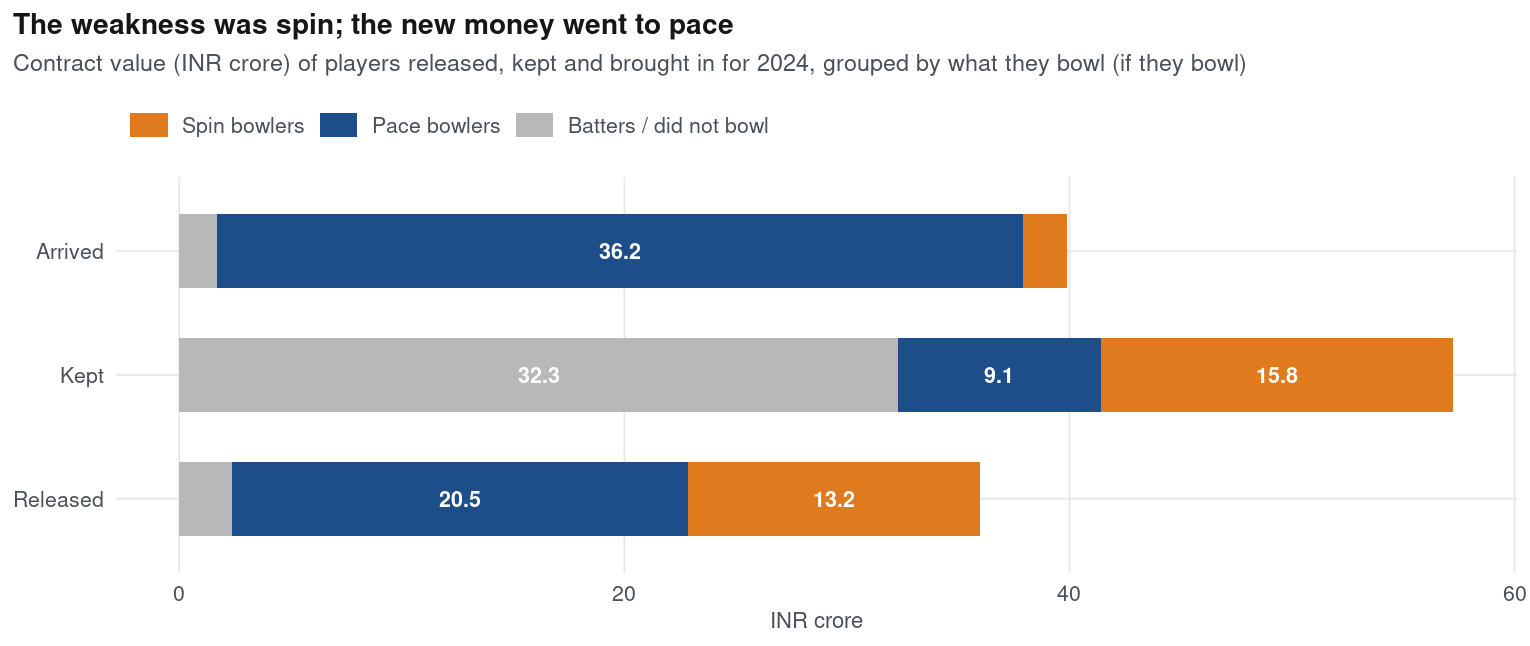
\includegraphics[width=\linewidth]{c04_money_moves.png}
\caption{Contract value released, kept and brought in for 2024, by what the player bowls.}
\label{fig:money}
\end{figure}

\textbf{Problem B: decision audit.} The gap cost \kv{stakerunsa} runs (\kv{stakewinsa} wins, INR~\kv{stakecra} crore) in 2023 and \kv{stakerunsb} in 2024. The franchise released \kv{releasedspinlist} and put INR~\kv{pacenew} crore of new money into pace and INR~\kv{spinnew} crore into spin (\cref{fig:money}). Arrivals produced \kv{wararrived24} WAR in 2024 against \kv{warreleased24} for those released, at INR~\kv{cpwarrived24} crore per WAR. The December 2023 pool held only \kv{marketpooln} spinners with any 2023 middle-overs evidence; the established ones were retained elsewhere, reachable only by trade. On 2023 evidence alone the best candidate projected only \kv{foremaxwins} wins better than the team's own; in hindsight \kv{besthindplayer} would have saved \kv{besthindruns} runs (\kv{besthindwins} wins). Within 2024 the team went from \kv{elWa} win in \kv{elMa} to \kv{elWb} in \kv{elMb}, with powerplay wickets \kv{elppwktsa}$\to$\kv{elppwktsb}; middle-overs spin economy moved only from \kv{elmidspinecona} to \kv{elmidspineconb}.

\begin{figure}[t]
\centering
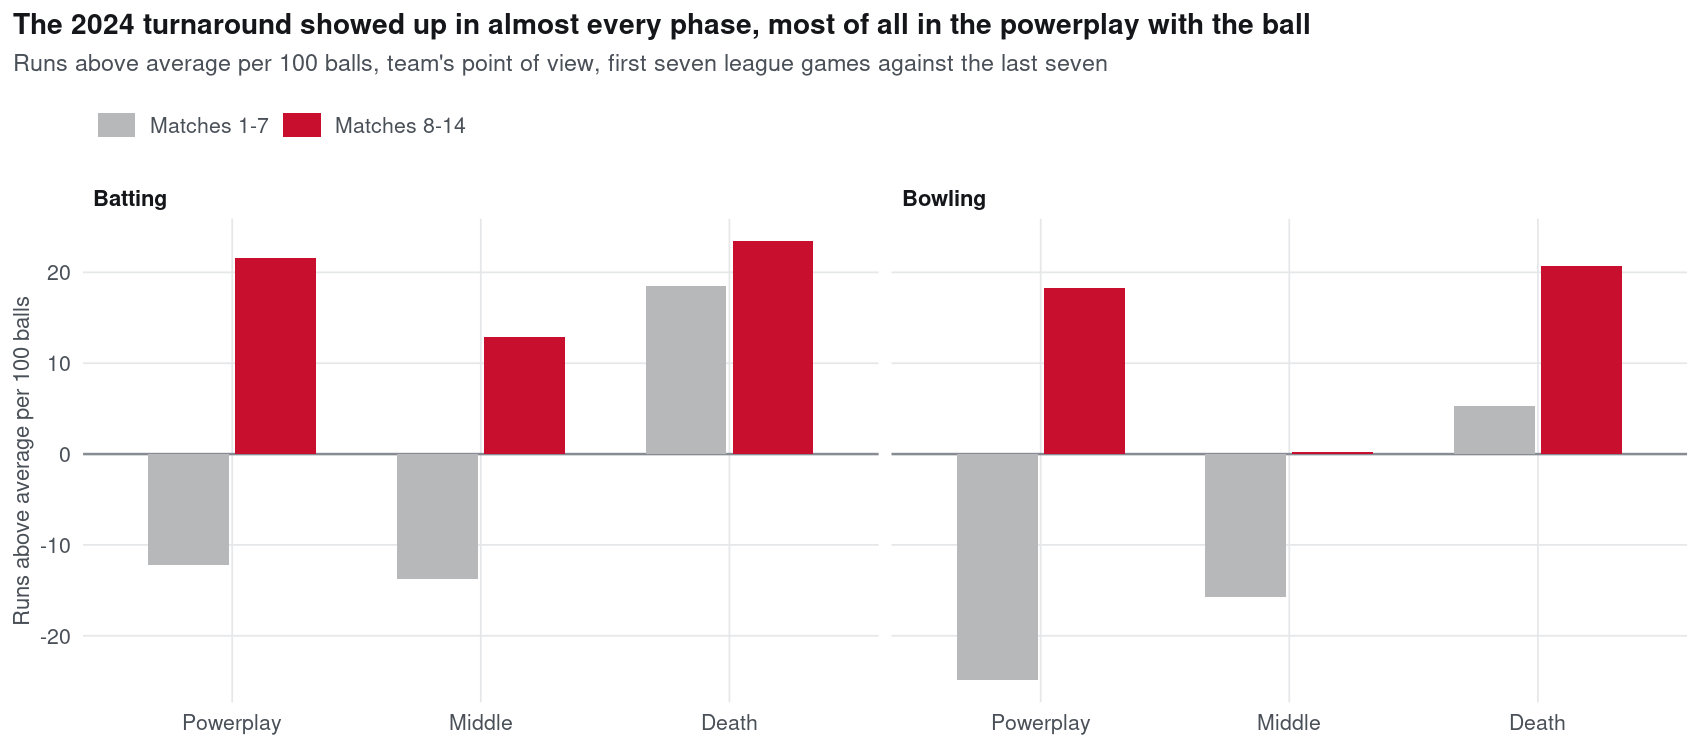
\includegraphics[width=\linewidth]{c08_early_late.png}
\caption{2024 league stage: runs above average per 100 balls by phase, first seven games against the last seven.}
\label{fig:el}
\end{figure}

\section{Decision}
\begin{table}[t]
\centering\footnotesize
\begin{tabular}{@{}lrrrr@{}}
\toprule
Option & E[wins] & 5\% & 95\% & P$>$0 \% \\
\midrule
\oprows
\bottomrule
\end{tabular}
\caption{Simulated wins per season on shrunk projections.}
\label{tab:options}
\end{table}
Recoverable value is smaller than the measured cost because individual estimates are heavily shrunk (\cref{tab:options}): a top-quartile Indian middle-overs spinner adds \kv{optC} wins (\kv{optCp}\% chance positive), up to \kv{histupper} if the gap repeated. We recommend redeploying middle overs to the positive options now and buying one Indian middle-overs spinner on more than one season of evidence, with a bid ceiling of projected WAR at the league rate, and not spending premium or overseas slots on more pace or on ``clutch''. Unused in the analysis: at the 2025 auction the franchise bought two spinners, one of them third on our shortlist.

\section{Limitations}
Two seasons support direction more than size; G1 is uncertain under resampling; prices for some replacement signings are missing; the audit is descriptive, not causal; and WAR levels depend on the stated replacement and runs-per-win choices.

{\small
\bibliographystyle{ieeenat_fullname}
\bibliography{refs}
}
\end{document}
